\section{Results}\label{sec:results}

\begin{figure}[t]
	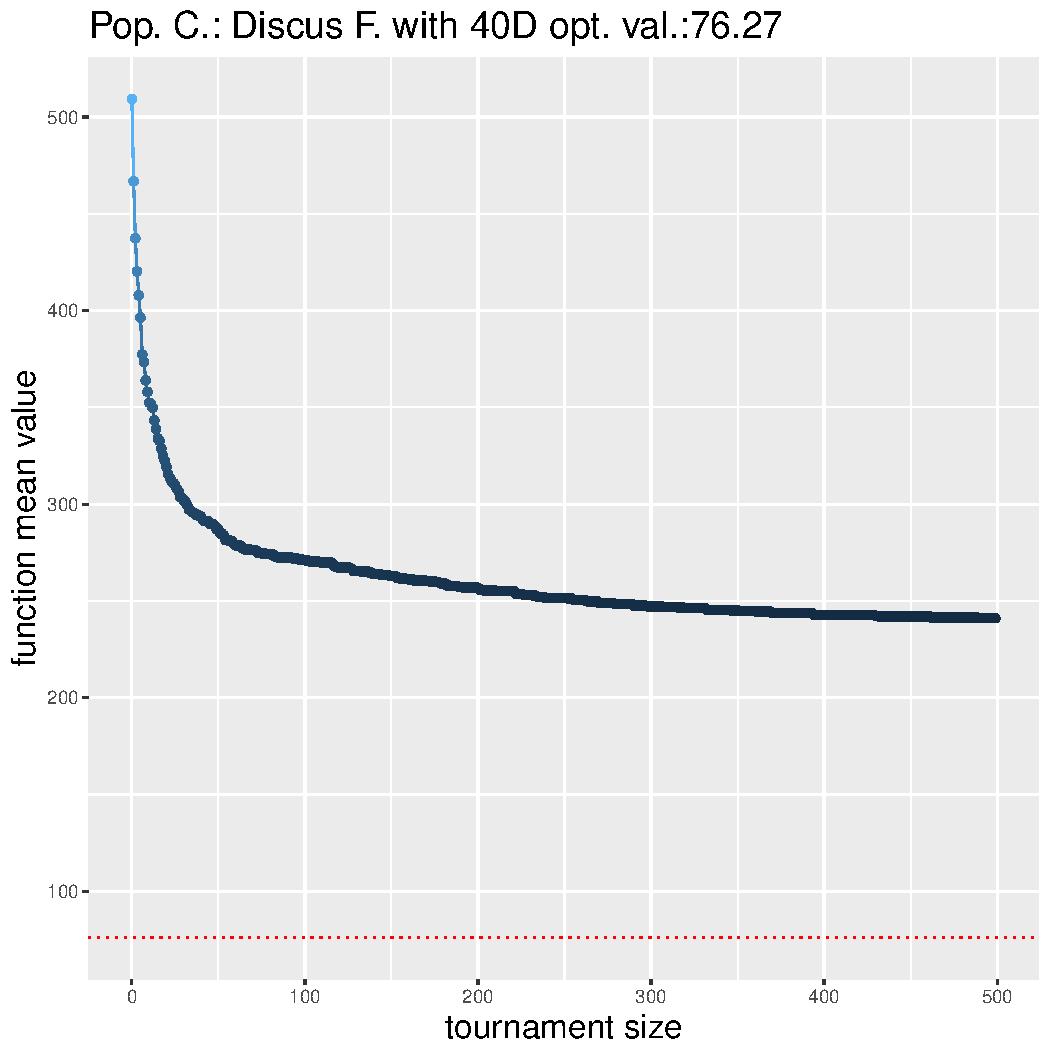
\includegraphics[width=0.45\textwidth]{img/SBX-40D/covergency_unimodal_sbx_11_dim_40.pdf}
	\caption{Population convergence for Discus Function with the SBX crossover - ($\lambda, \lambda$) scheme.}
	\label{convergence-sbx-11-a}
\end{figure}

\begin{figure}[t]
	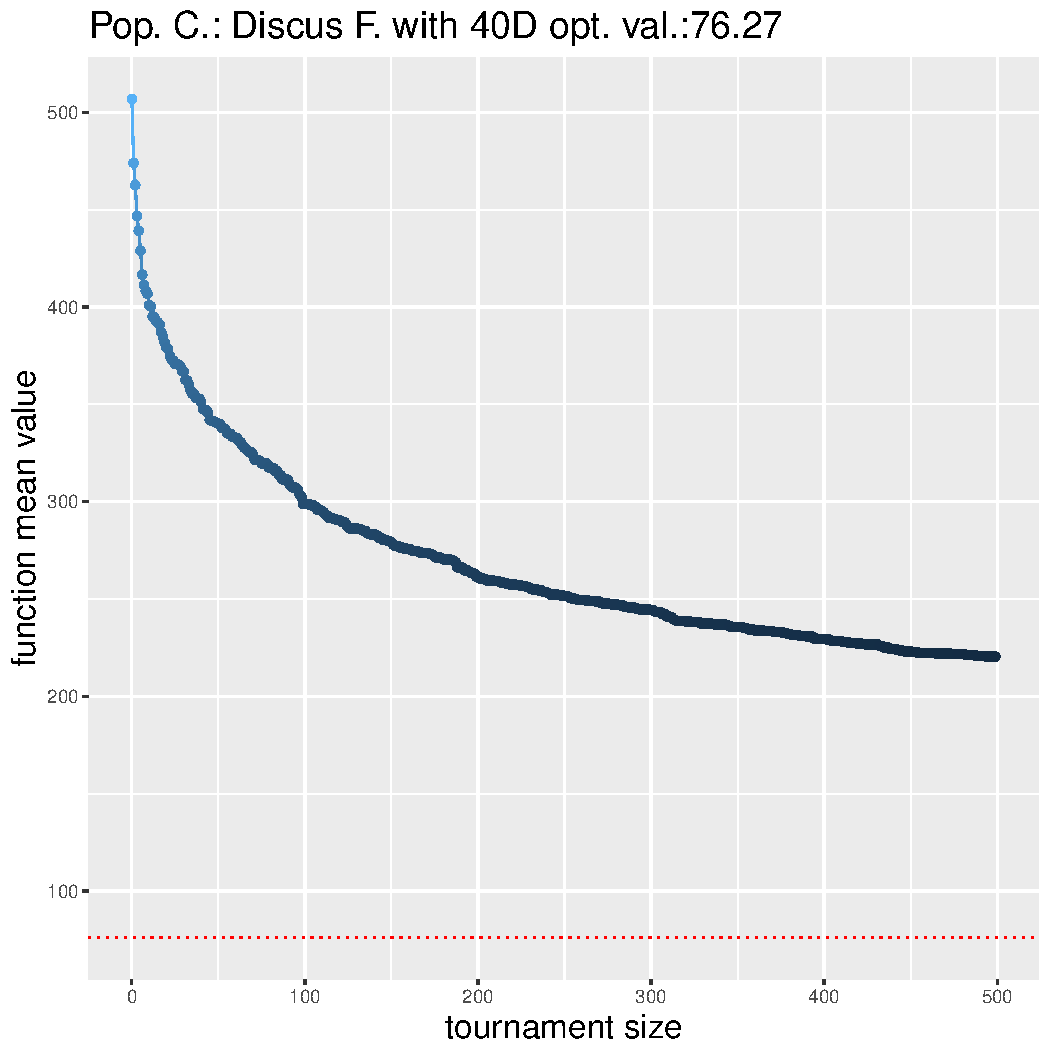
\includegraphics[width=0.45\textwidth]{img/uniform-40D/covergency_unimodal_uniform_11_dim_40.pdf}
	\caption{Population convergence for Discus Function with the uniform crossover - ($\lambda, \lambda$) scheme.}
	\label{convergence-uniform-11-a}
\end{figure}


\begin{figure}[t]
	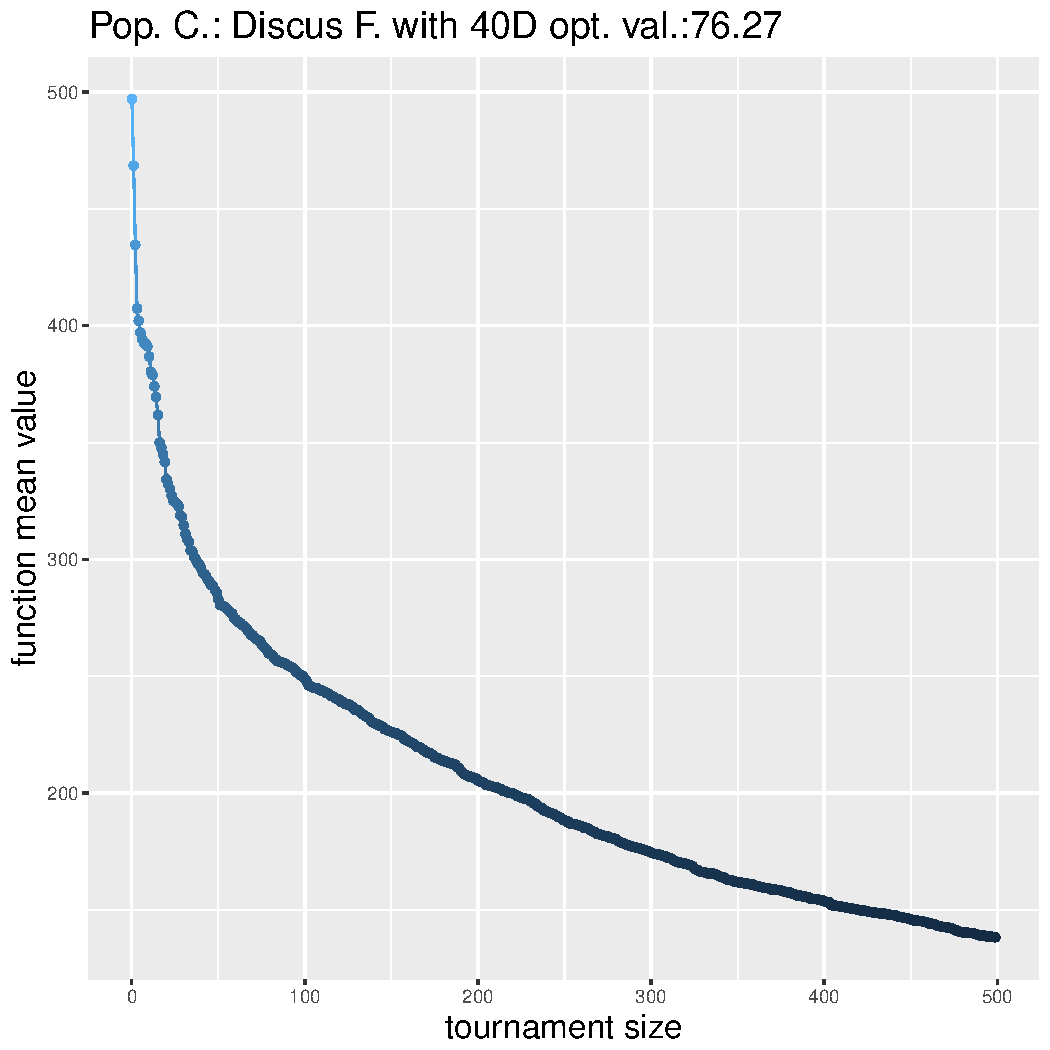
\includegraphics[width=0.45\textwidth]{img/2n2n-40D/covergency_unimodal_2n2n_11_dim_40.pdf}
	\caption{Population convergence for Discus Function - ($\lambda + \lambda$) scheme with the SBX crossover - ($\lambda + \lambda$) scheme.}
	\label{convegence-11-b}
\end{figure}


\begin{figure*}[t]
	\begin{subfigure}[b]{0.33\textwidth}
		\centering
		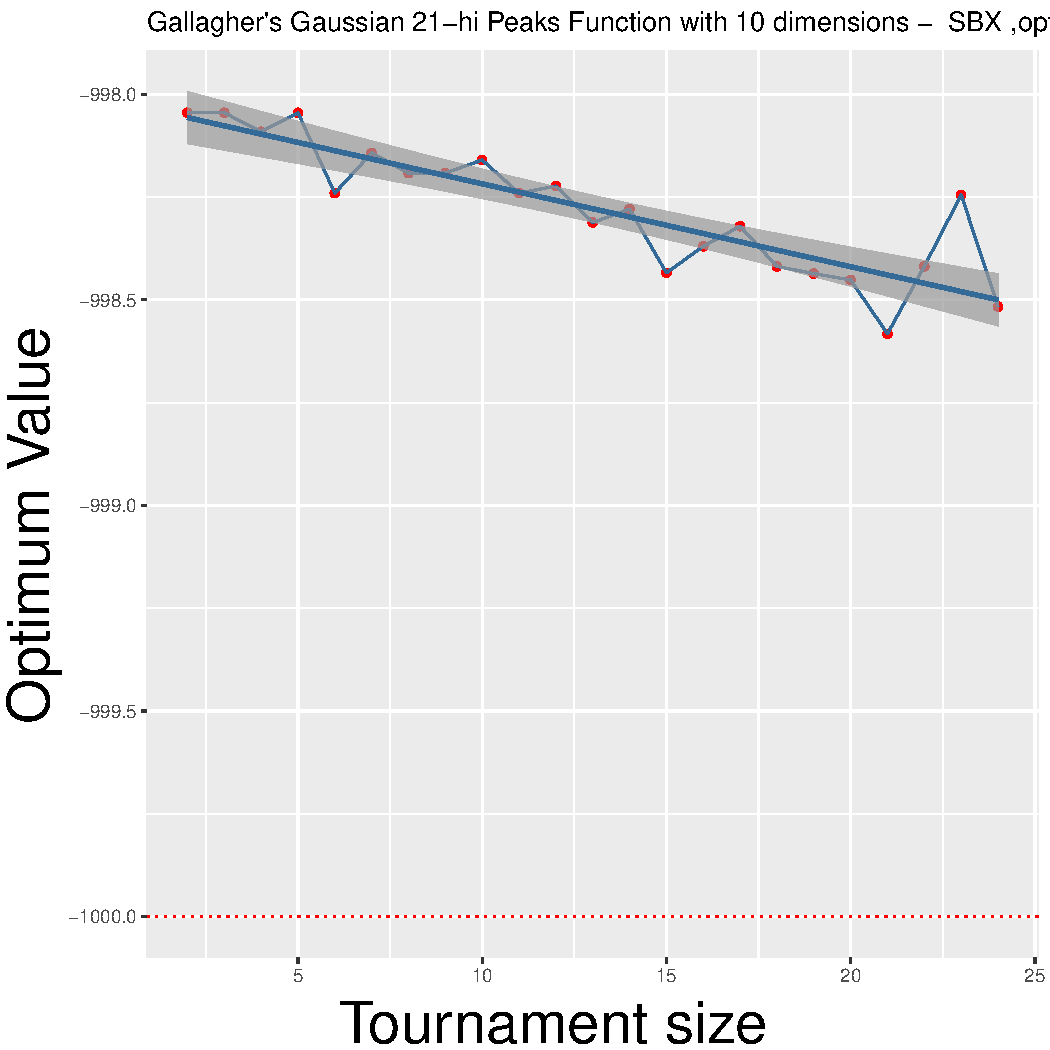
\includegraphics[width=\textwidth]{img/SBX-10D/multimodal_sbx_22_dim_10.pdf}
		\caption{10 dimensions.}
	\end{subfigure}
	\begin{subfigure}[b]{0.33\textwidth}
		\centering
		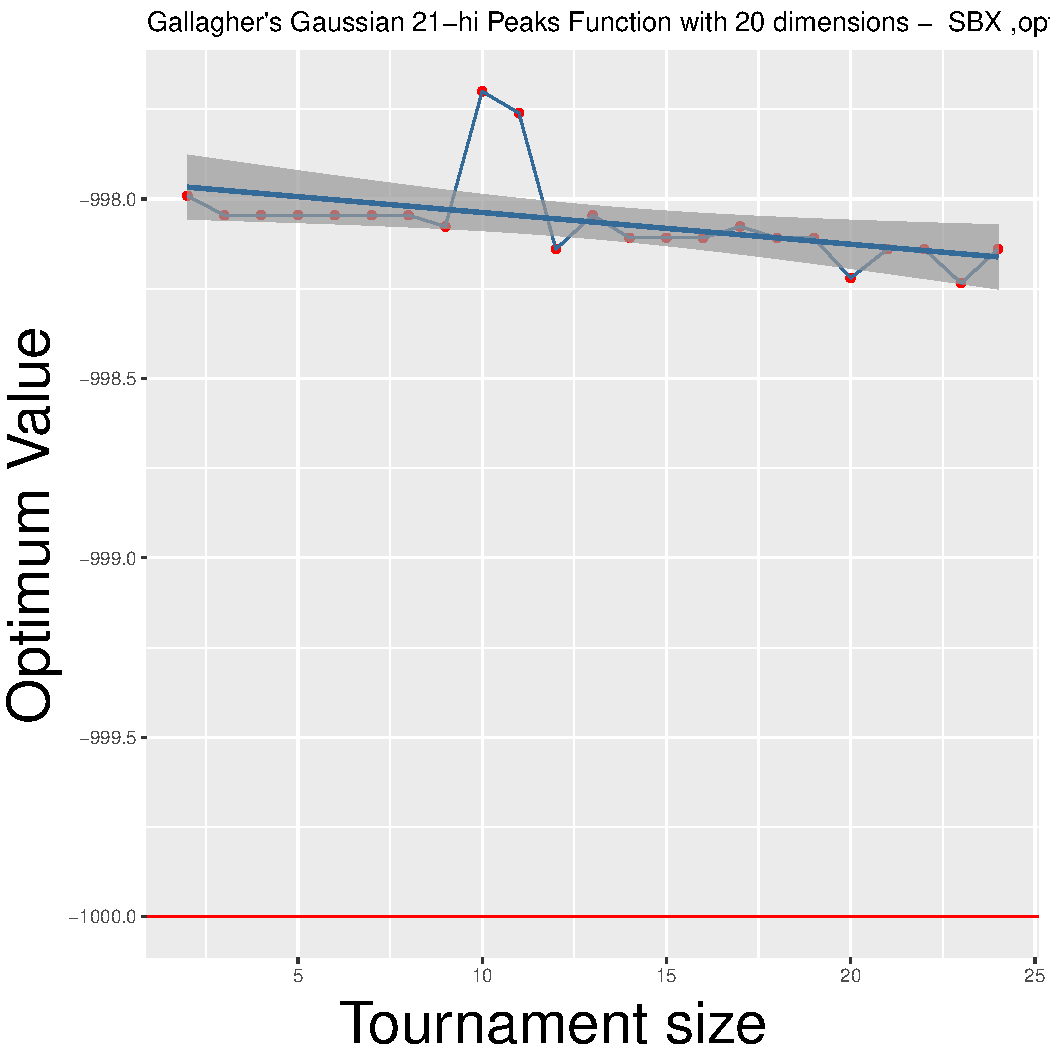
\includegraphics[width=\textwidth]{img/SBX-20D/multimodal_sbx_22_dim_20.pdf}
		\caption{20 dimensions.}
	\end{subfigure}
	\begin{subfigure}[b]{0.33\textwidth}
		\centering
		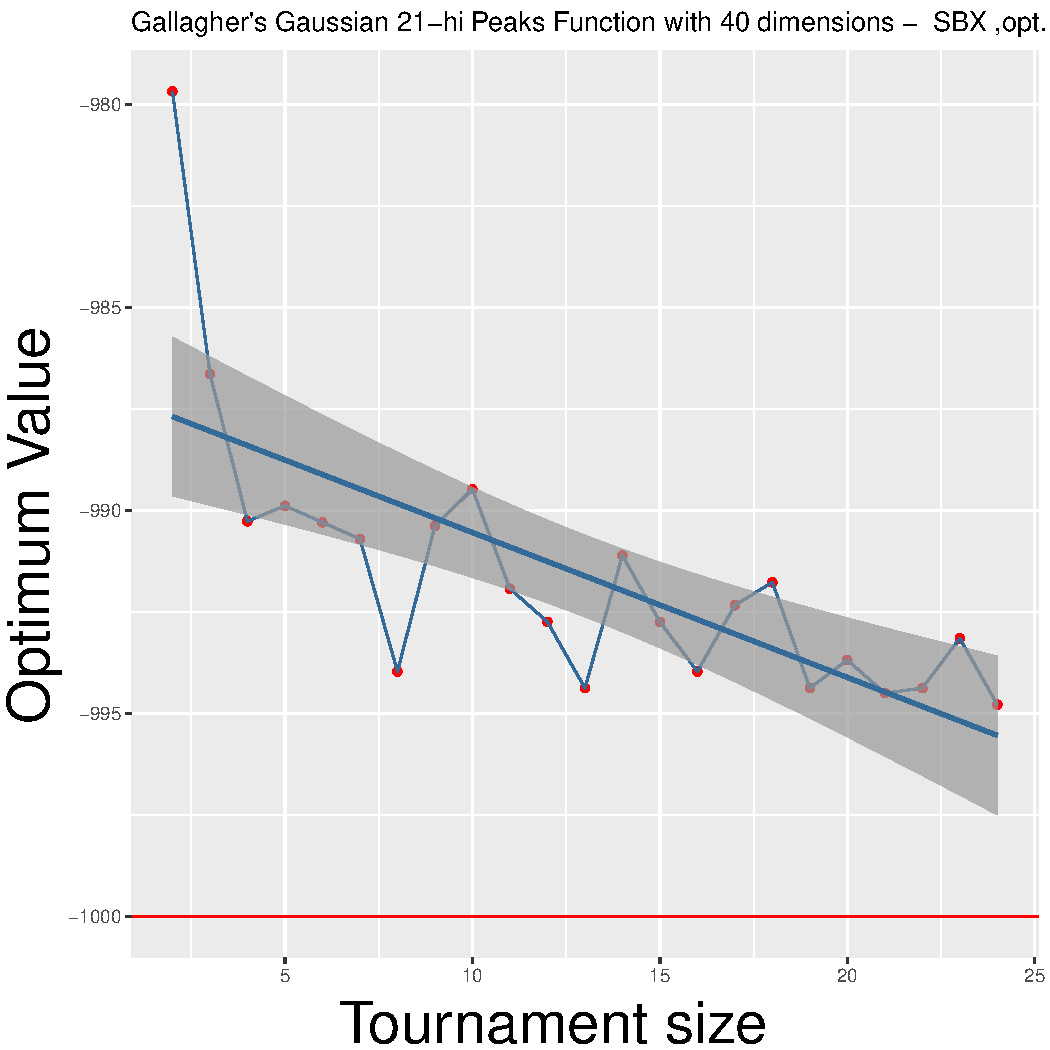
\includegraphics[width=\textwidth]{img/SBX-40D/multimodal_sbx_22_dim_40.pdf}
		\caption{40 dimensions.}
	\end{subfigure}
	\caption{Average performance on different tournament size for the Gallagher's Gaussian 21-hi Peaks Function, when using the SBX crossover - ($\lambda, \lambda$) scheme.}
	\label{sbx-22-a}
	\begin{subfigure}[b]{0.33\textwidth}
		\centering
		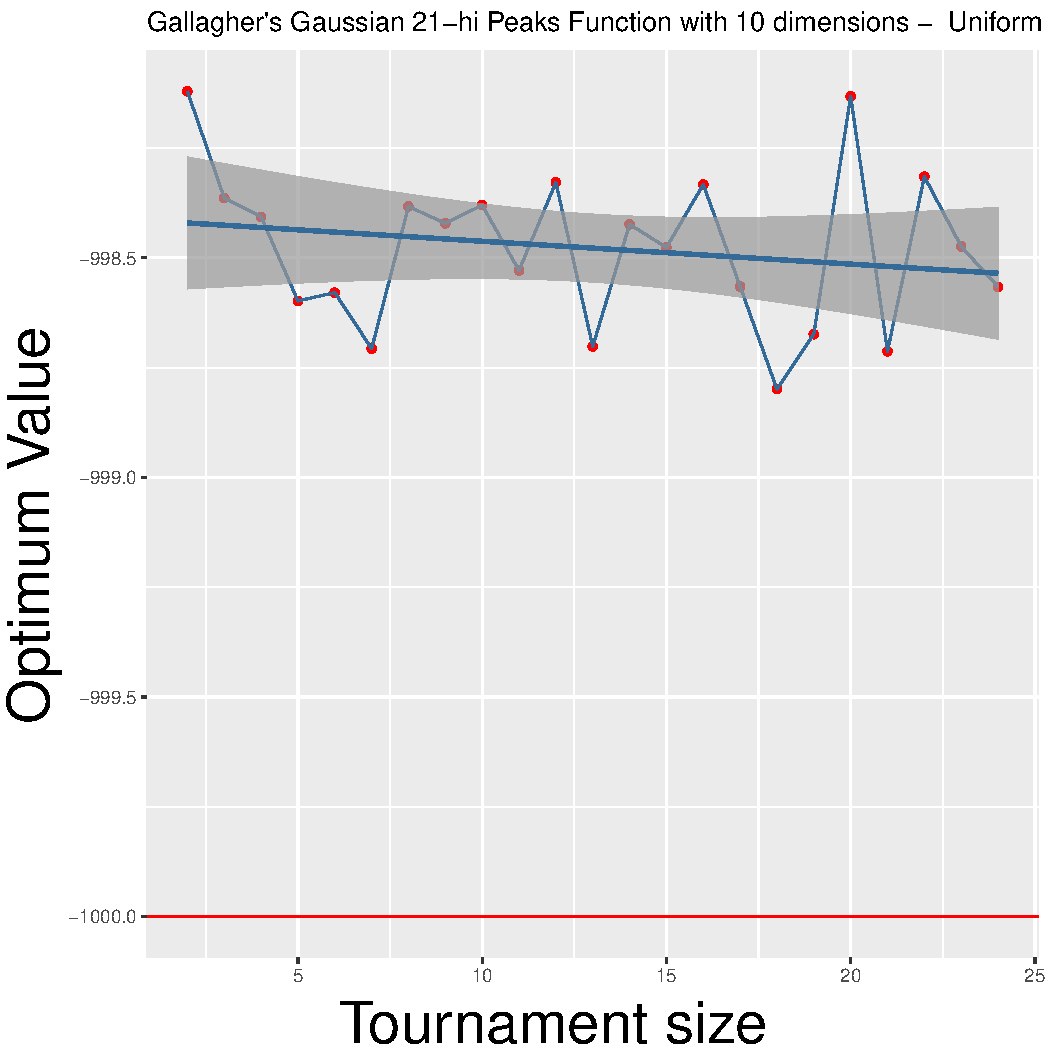
\includegraphics[width=\textwidth]{img/uniform-10D/multimodal_uniform_22_dim_10.pdf}
		\caption{10 dimensions.}
	\end{subfigure}
	\begin{subfigure}[b]{0.33\textwidth}
		\centering
		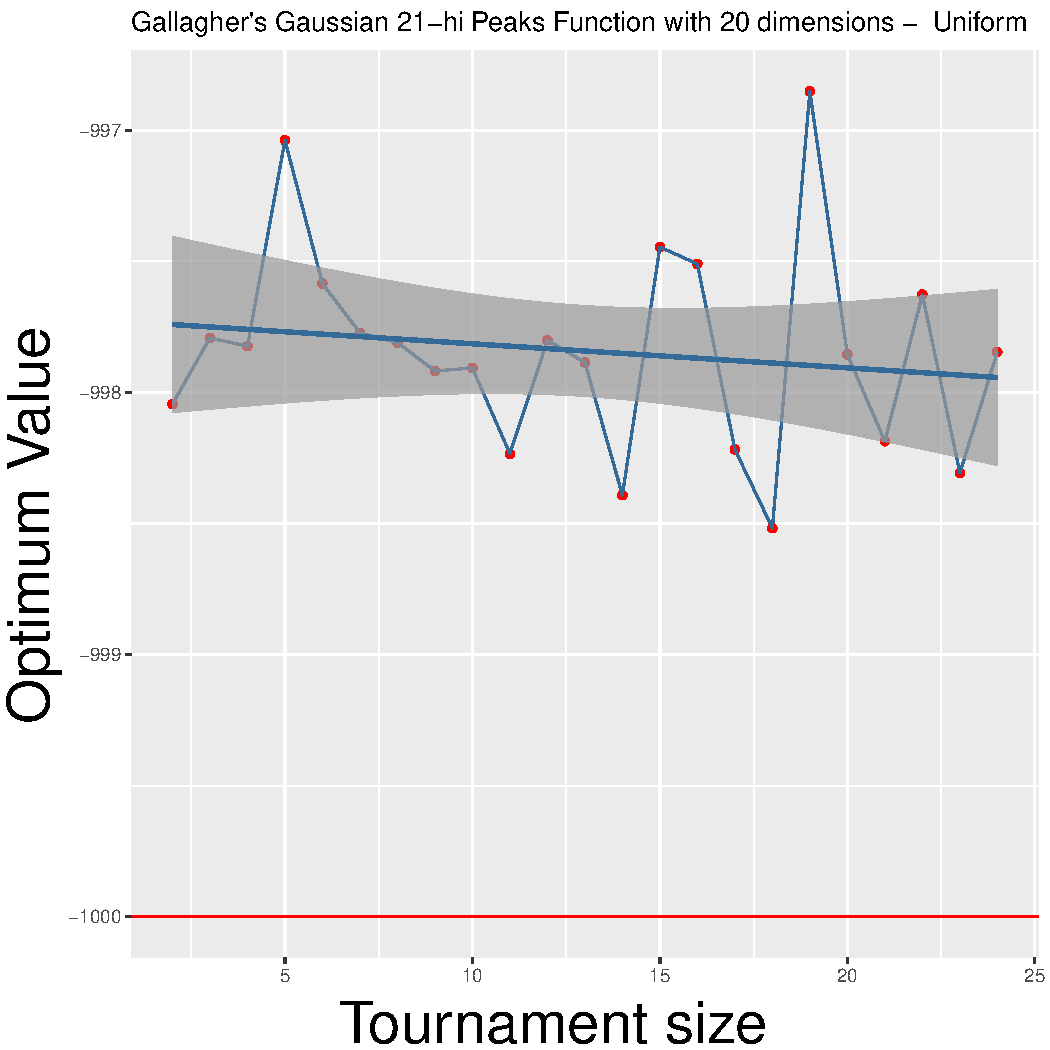
\includegraphics[width=\textwidth]{img/uniform-20D/multimodal_uniform_22_dim_20.pdf}
		\caption{20 dimensions.}
	\end{subfigure}
	\begin{subfigure}[b]{0.33\textwidth}
		\centering
		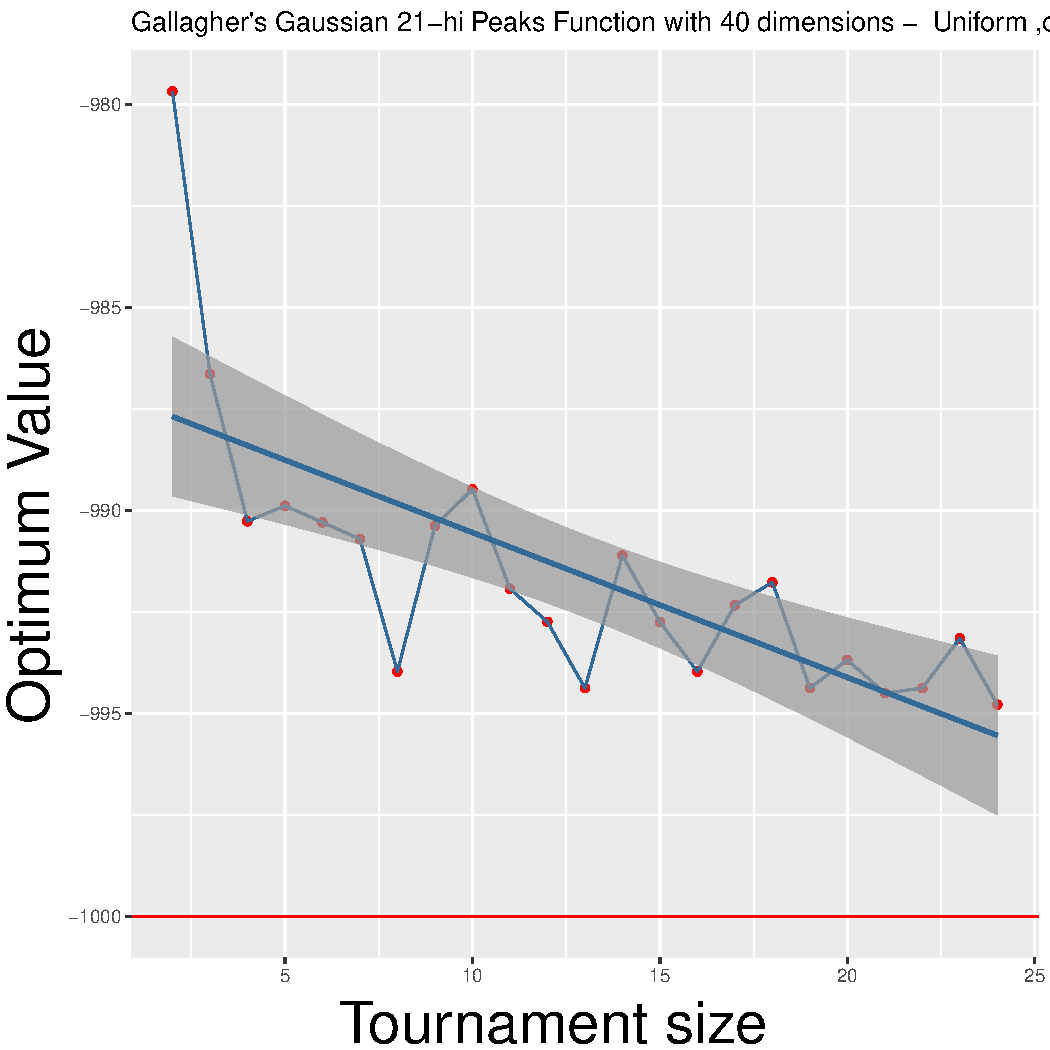
\includegraphics[width=\textwidth]{img/uniform-40D/multimodal_uniform_22_dim_40.pdf}
		\caption{40 dimensions.}
	\end{subfigure}
	\caption{Average performance on different tournament size for the Gallagher's Gaussian 21-hi Peaks Function, when using the uniform crossover - ($\lambda, \lambda$) scheme.}
	\label{uniform-22-a}
	\begin{subfigure}[b]{0.33\textwidth}
		\centering
		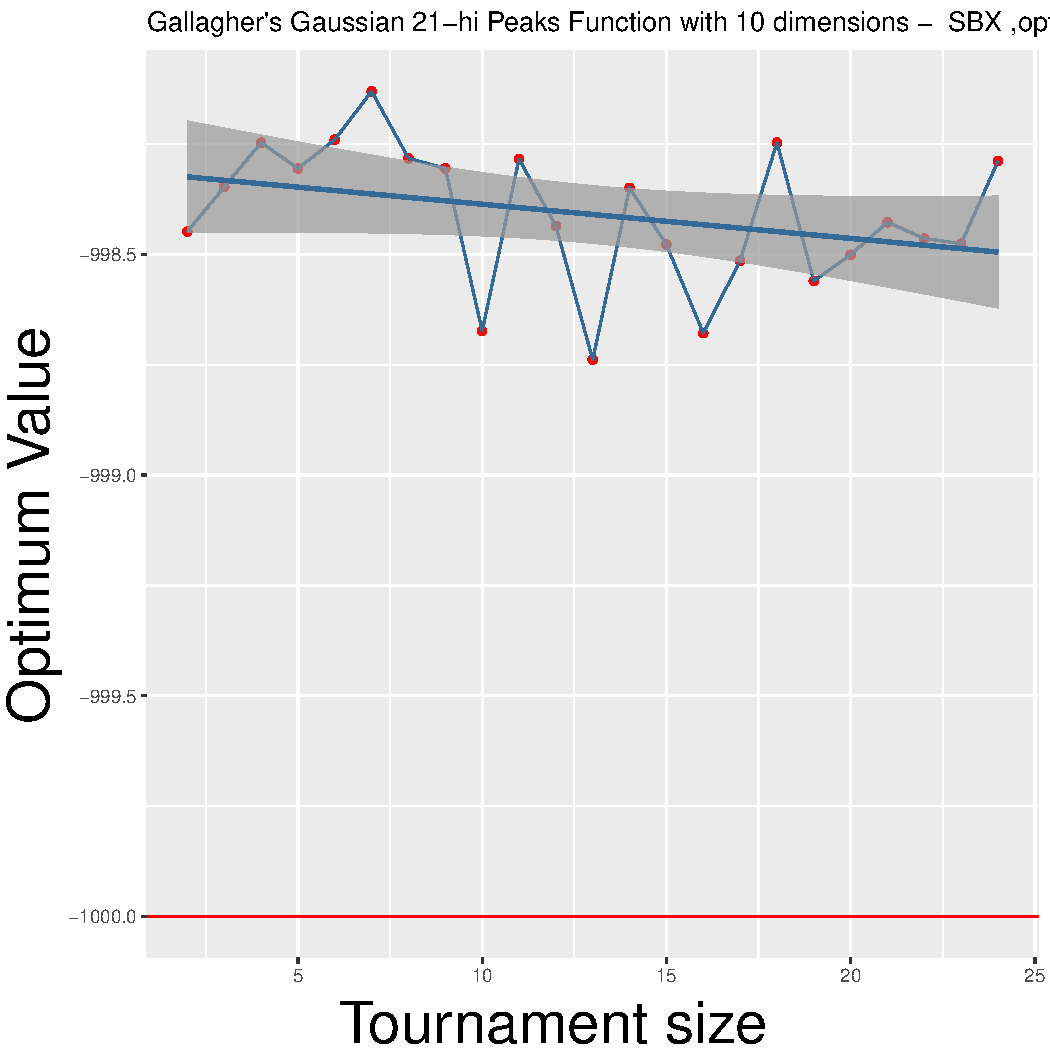
\includegraphics[width=\textwidth]{img/2n2n-10D/multimodal_2n2n_22_dim_10.pdf}
		\caption{10 dimensions.}
	\end{subfigure}
	\begin{subfigure}[b]{0.33\textwidth}
		\centering
		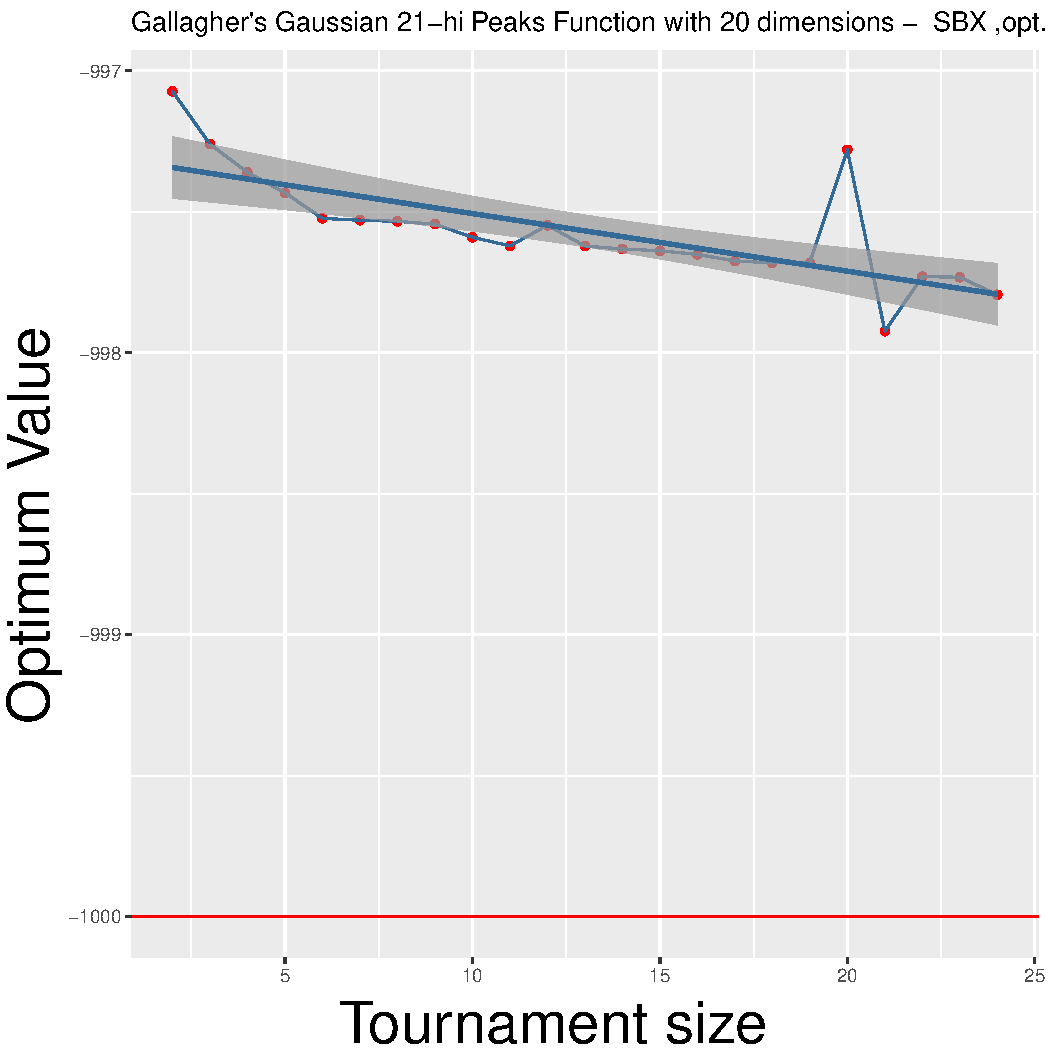
\includegraphics[width=\textwidth]{img/2n2n-20D/multimodal_2n2n_22_dim_20.pdf}
		\caption{20 dimensions.}
	\end{subfigure}
	\begin{subfigure}[b]{0.33\textwidth}
		\centering
		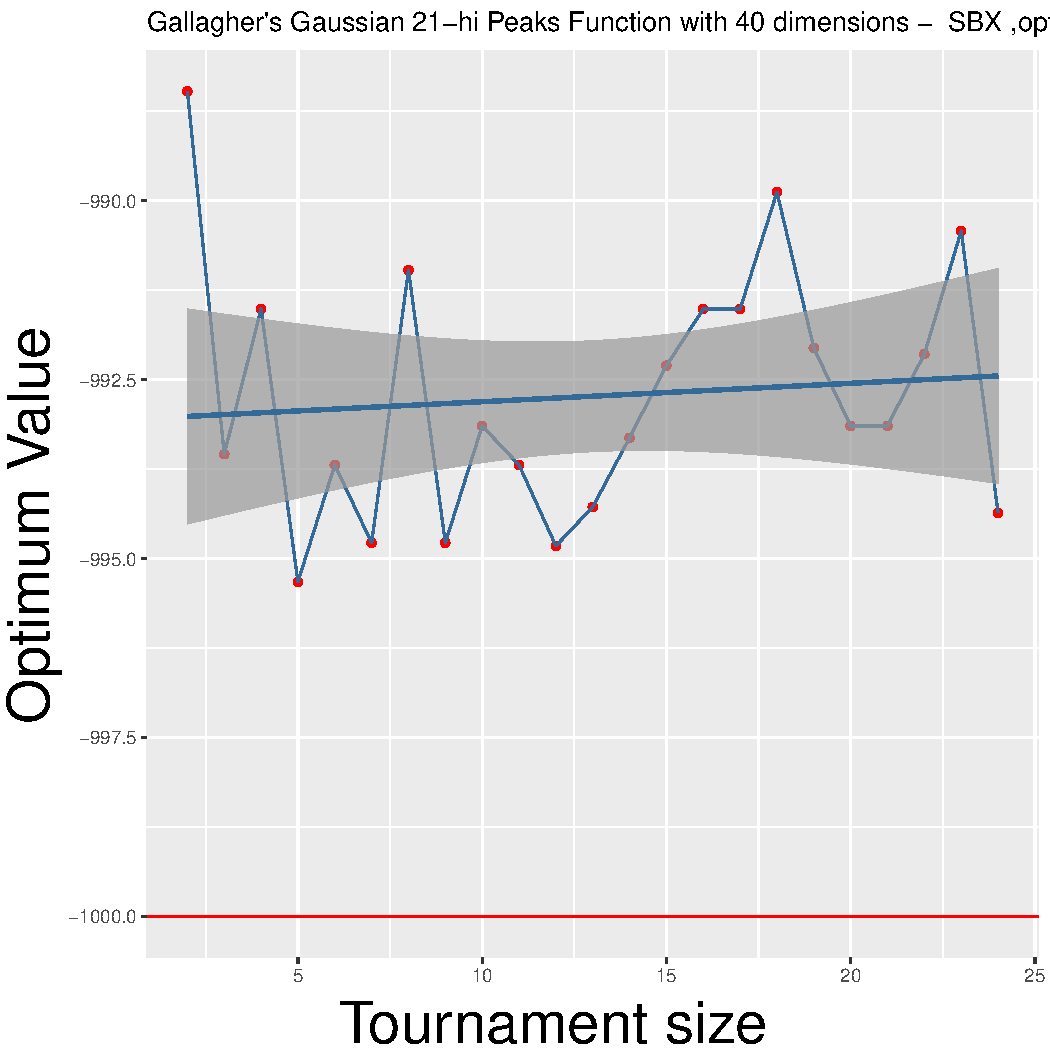
\includegraphics[width=\textwidth]{img/2n2n-40D/multimodal_2n2n_22_dim_40.pdf}
		\caption{40 dimensions.}
	\end{subfigure}
	\caption{Average performance on different tournament size for the Gallagher's Gaussian 21-hi Peaks Function, when using the SBX crossover - ($\lambda + \lambda$) scheme.}
	\label{sbx-22-B}
\end{figure*}


\begin{figure*}[t]
	\begin{subfigure}[b]{0.33\textwidth}
		\centering
		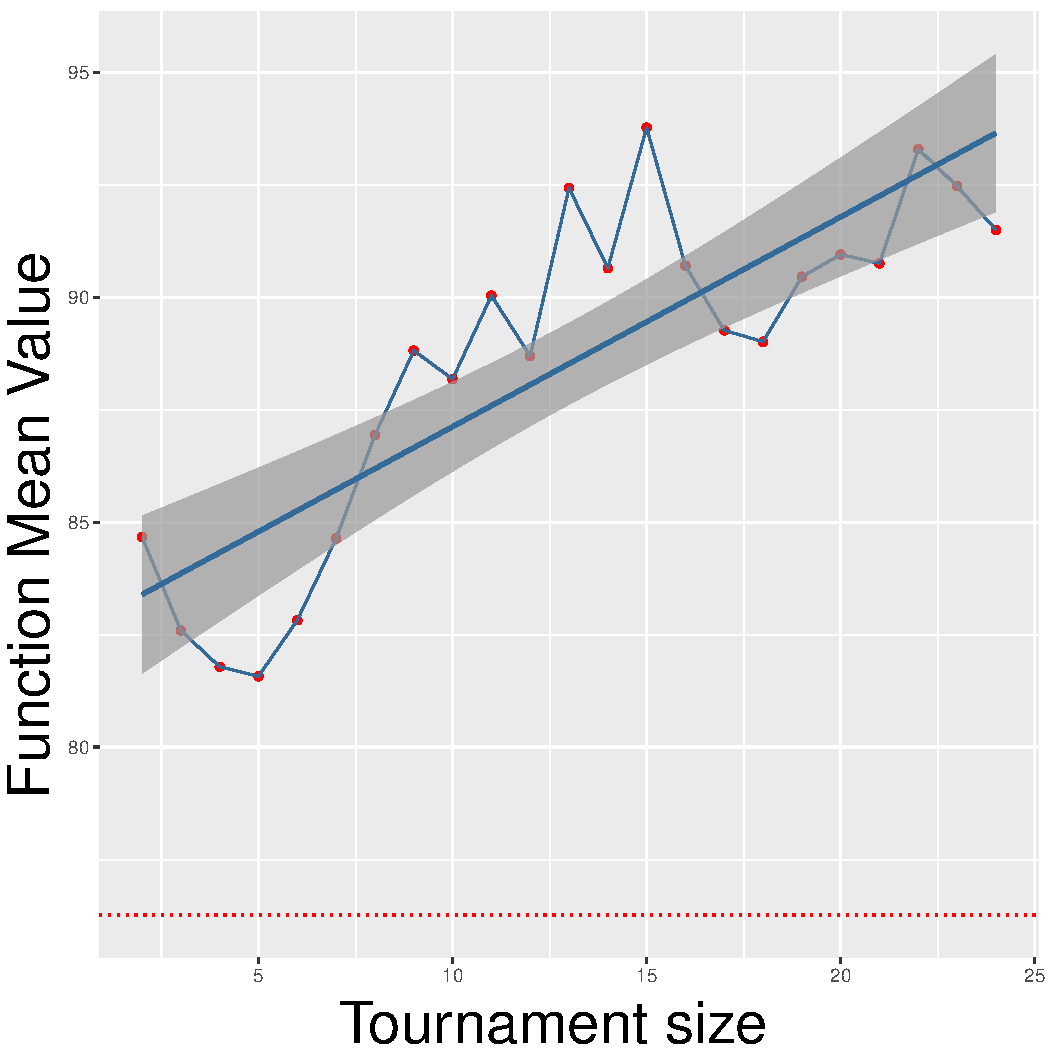
\includegraphics[width=\textwidth]{img/SBX-10D/unimodal_sbx_11_dim_10.pdf}
		\caption{10 dimensions.}
	\end{subfigure}
	\begin{subfigure}[b]{0.33\textwidth}
		\centering
		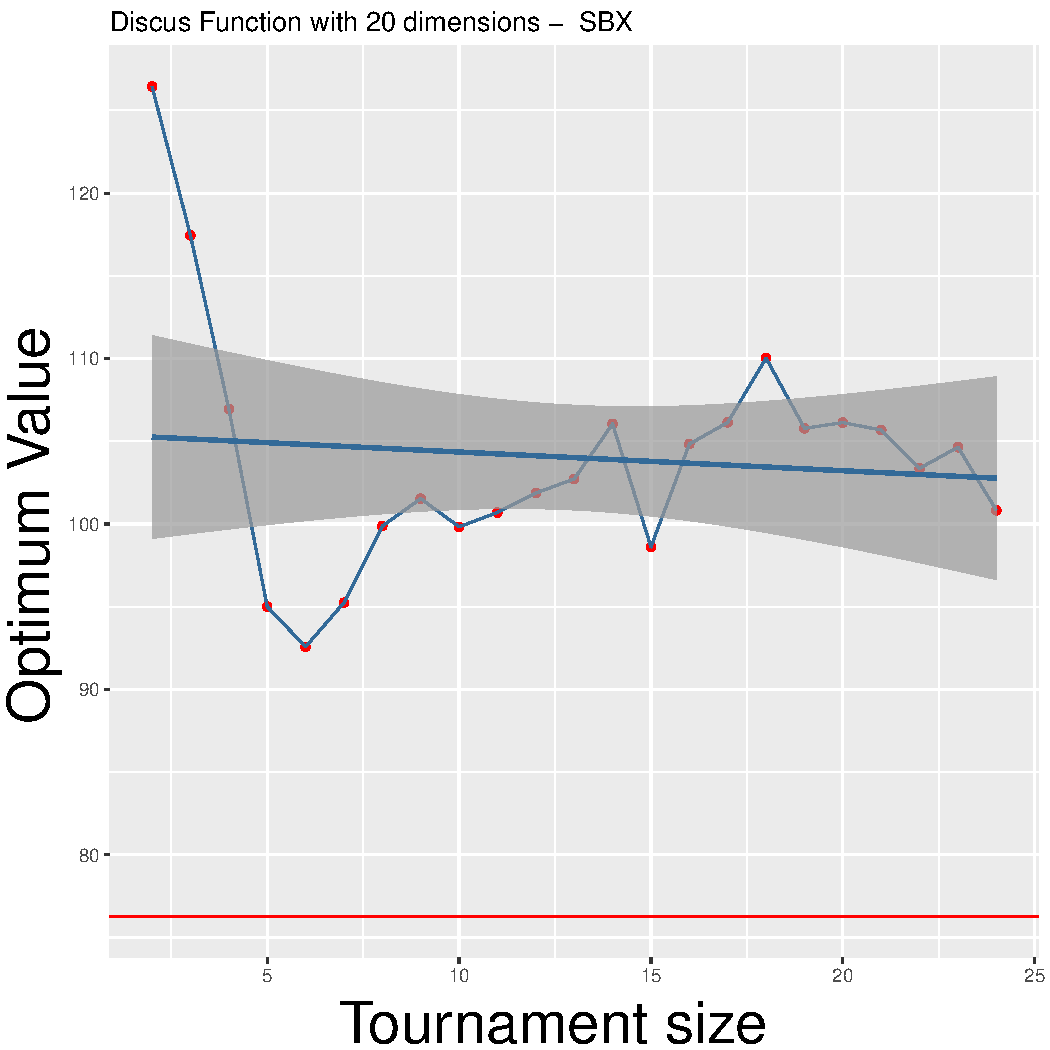
\includegraphics[width=\textwidth]{img/SBX-20D/unimodal_sbx_11_dim_20.pdf}
		\caption{20 dimensions.}
	\end{subfigure}
	\begin{subfigure}[b]{0.33\textwidth}
		\centering
		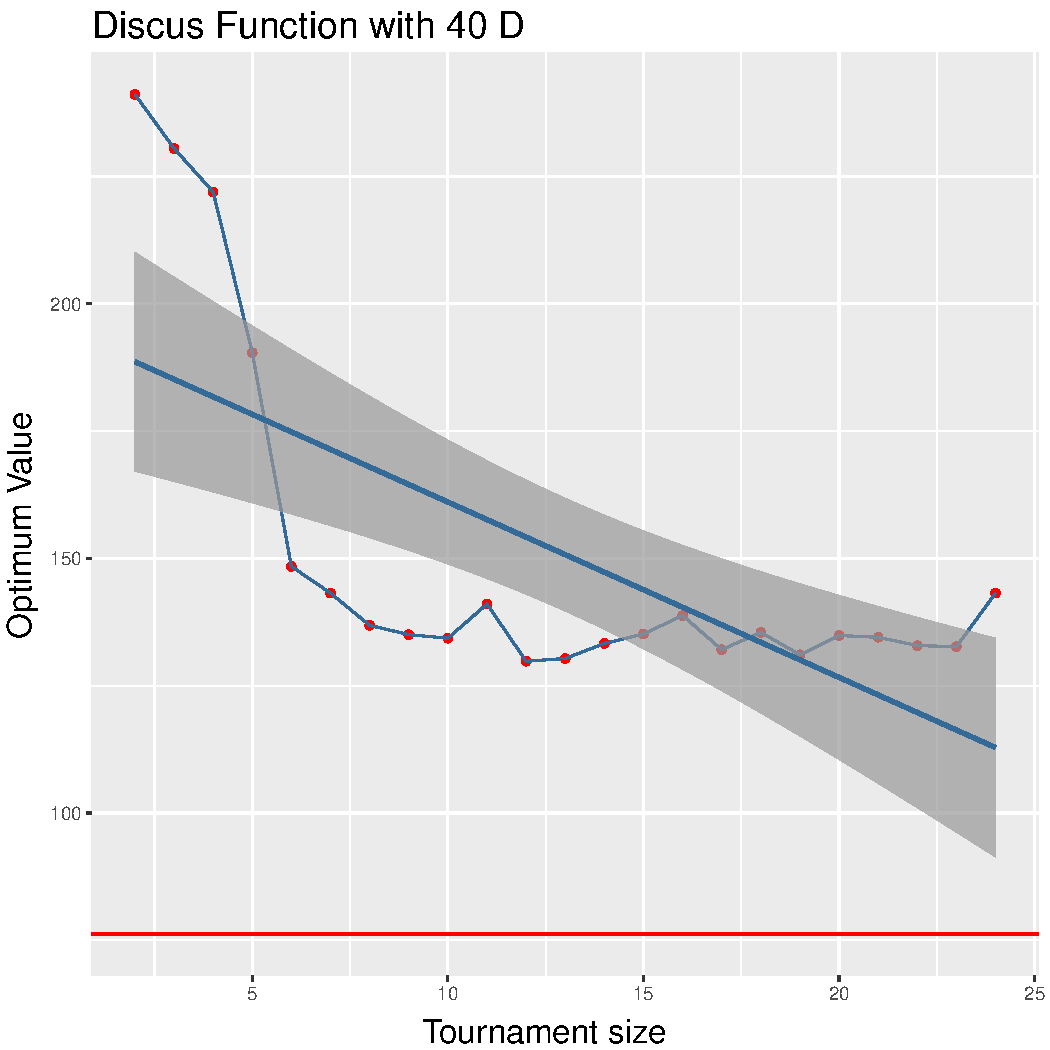
\includegraphics[width=\textwidth]{img/SBX-40D/unimodal_sbx_11_dim_40.pdf}
		\caption{40 dimensions.}
	\end{subfigure}
	\caption{Average performance on different tournament size for the Discus Function, when using the SBX crossover - ($\lambda, \lambda$) scheme.}
	\label{sbx-11-a}
	\begin{subfigure}[b]{0.33\textwidth}
		\centering
		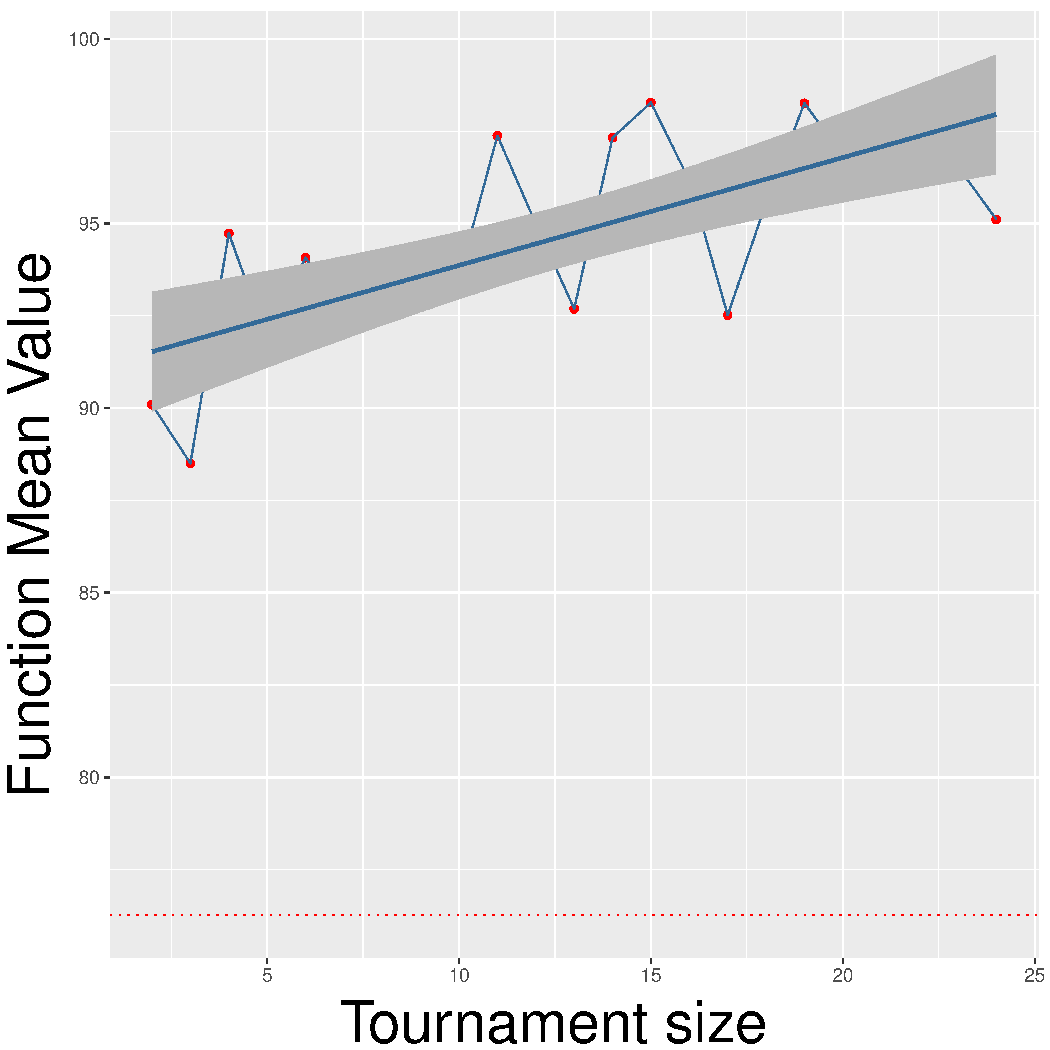
\includegraphics[width=\textwidth]{img/uniform-10D/unimodal_uniform_11_dim_10.pdf}
		\caption{10 dimensions.}
	\end{subfigure}
	\begin{subfigure}[b]{0.33\textwidth}
		\centering
		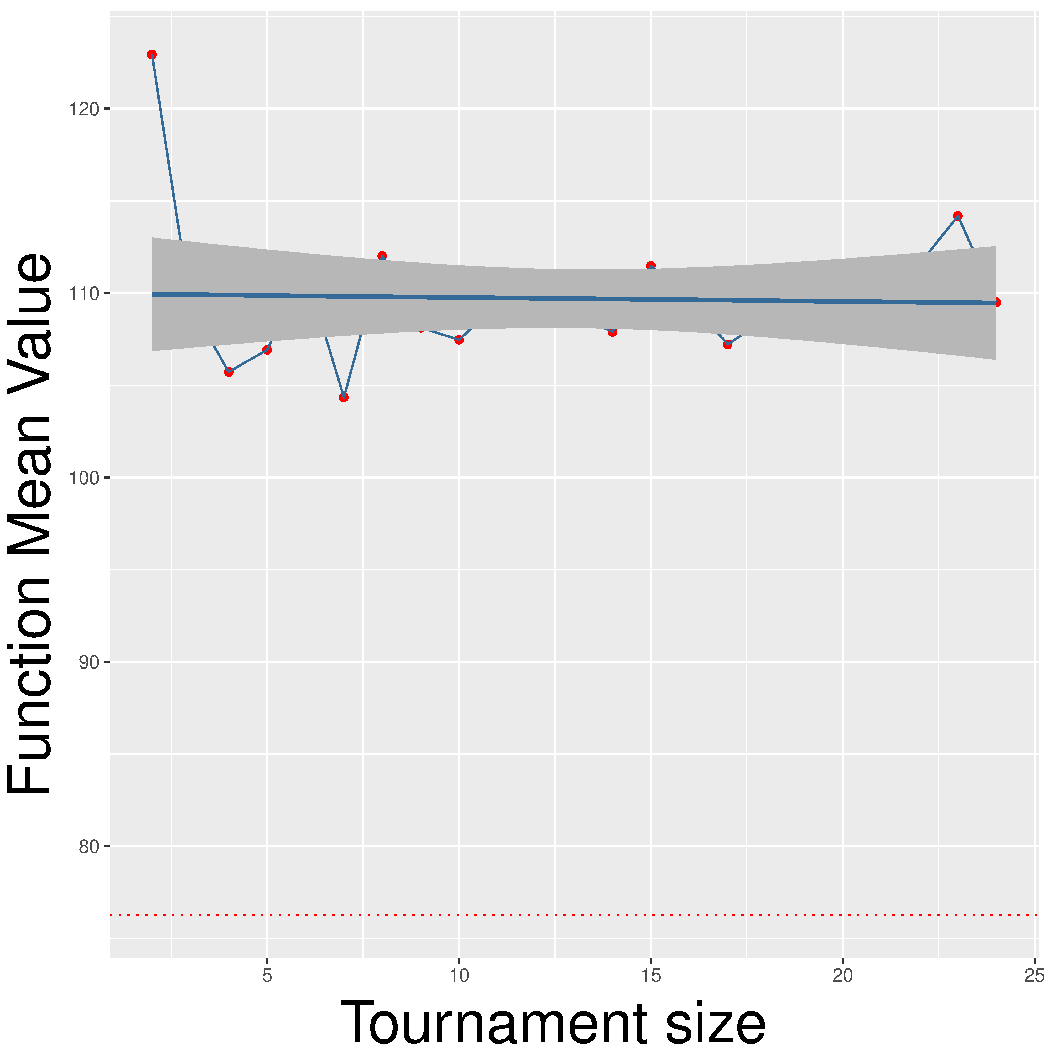
\includegraphics[width=\textwidth]{img/uniform-20D/unimodal_uniform_11_dim_20.pdf}
		\caption{20 dimensions.}
	\end{subfigure}
	\begin{subfigure}[b]{0.33\textwidth}
		\centering
		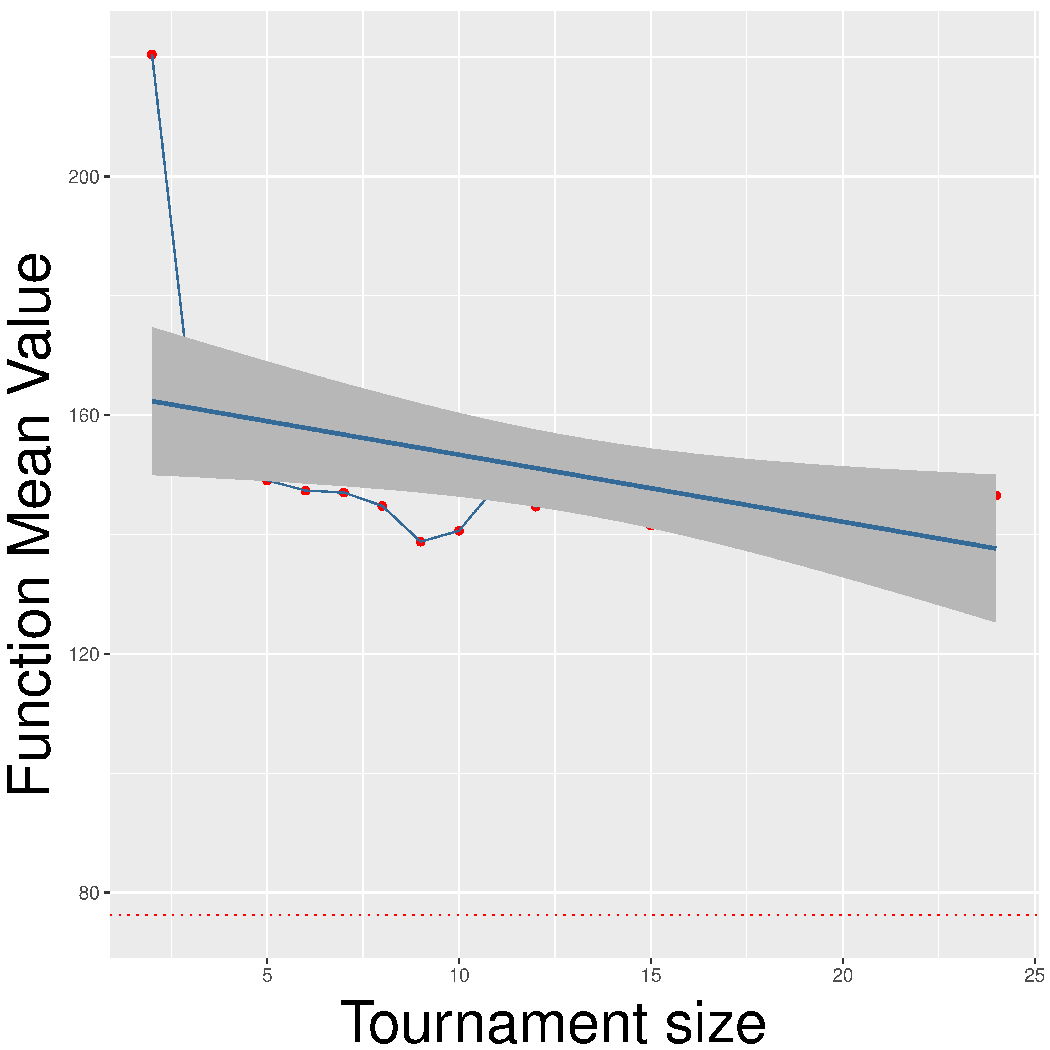
\includegraphics[width=\textwidth]{img/uniform-40D/unimodal_uniform_11_dim_40.pdf}
		\caption{40 dimensions.}
	\end{subfigure}
	\caption{Average performance on different tournament size for the Discus Function, when using the uniform crossover - ($\lambda, \lambda$) scheme.}
	\label{uniform-11-a}
	\begin{subfigure}[b]{0.33\textwidth}
		\centering
		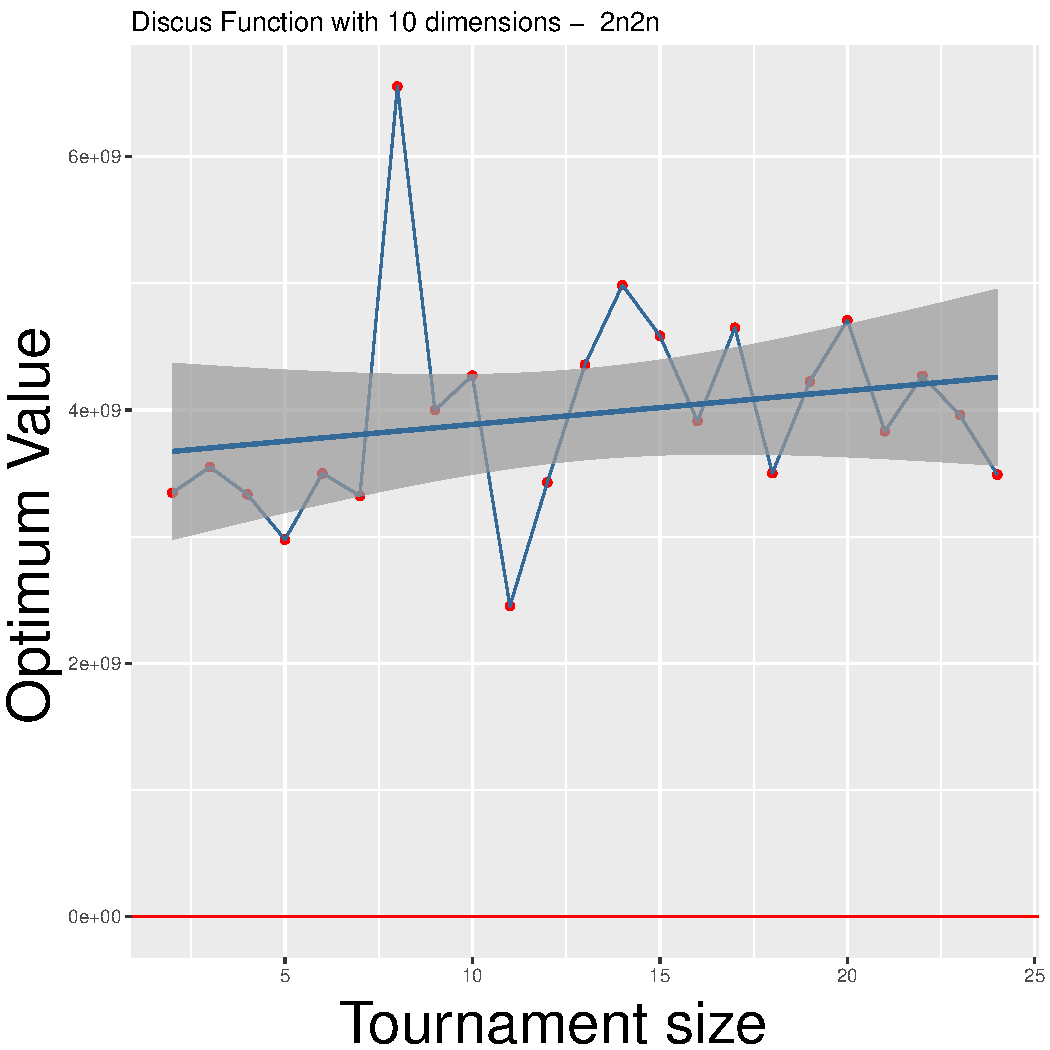
\includegraphics[width=\textwidth]{img/2n2n-10D/unimodal_2n2n_11_dim_10.pdf}
		\caption{10 dimensions.}
	\end{subfigure}
	\begin{subfigure}[b]{0.33\textwidth}
		\centering
		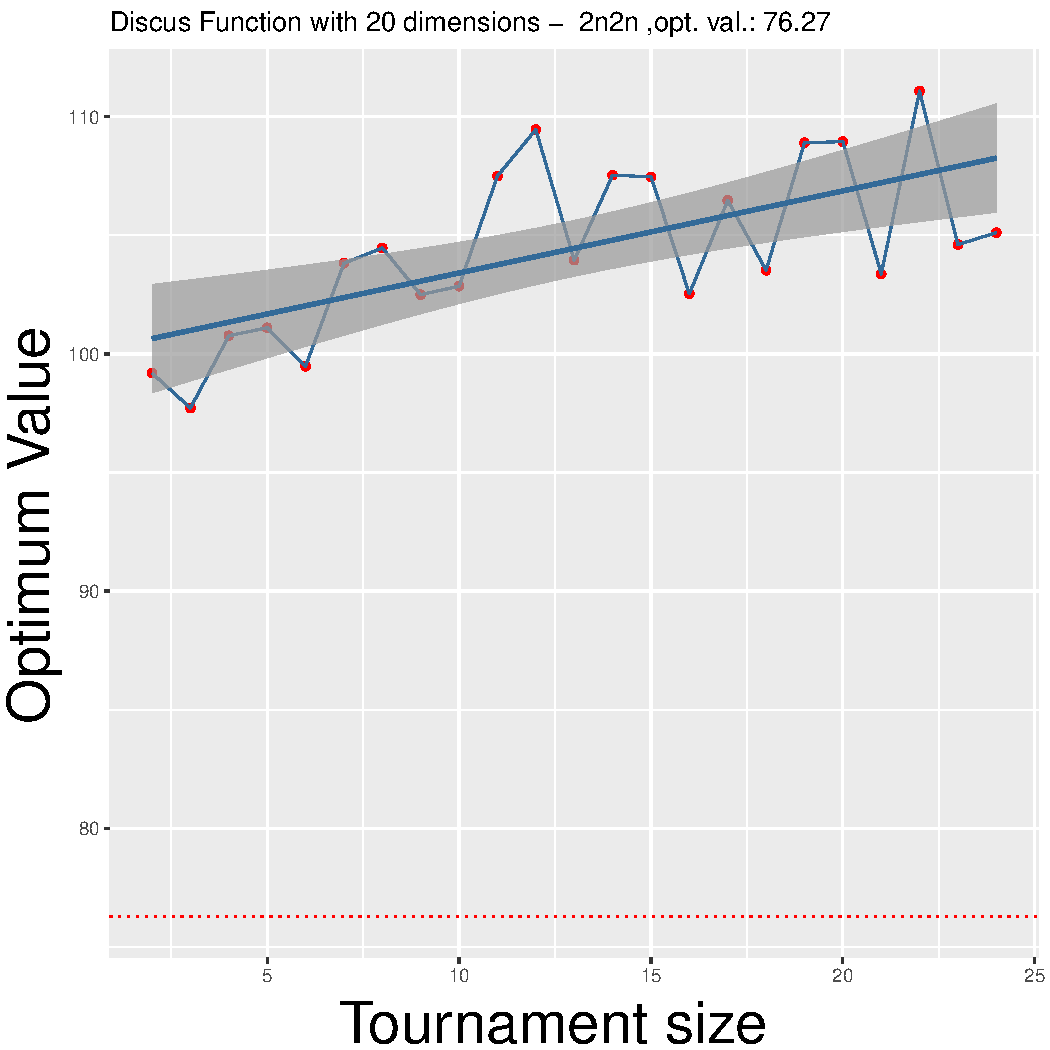
\includegraphics[width=\textwidth]{img/2n2n-20D/unimodal_2n2n_11_dim_20.pdf}
		\caption{20 dimensions.}
	\end{subfigure}
	\begin{subfigure}[b]{0.33\textwidth}
		\centering
		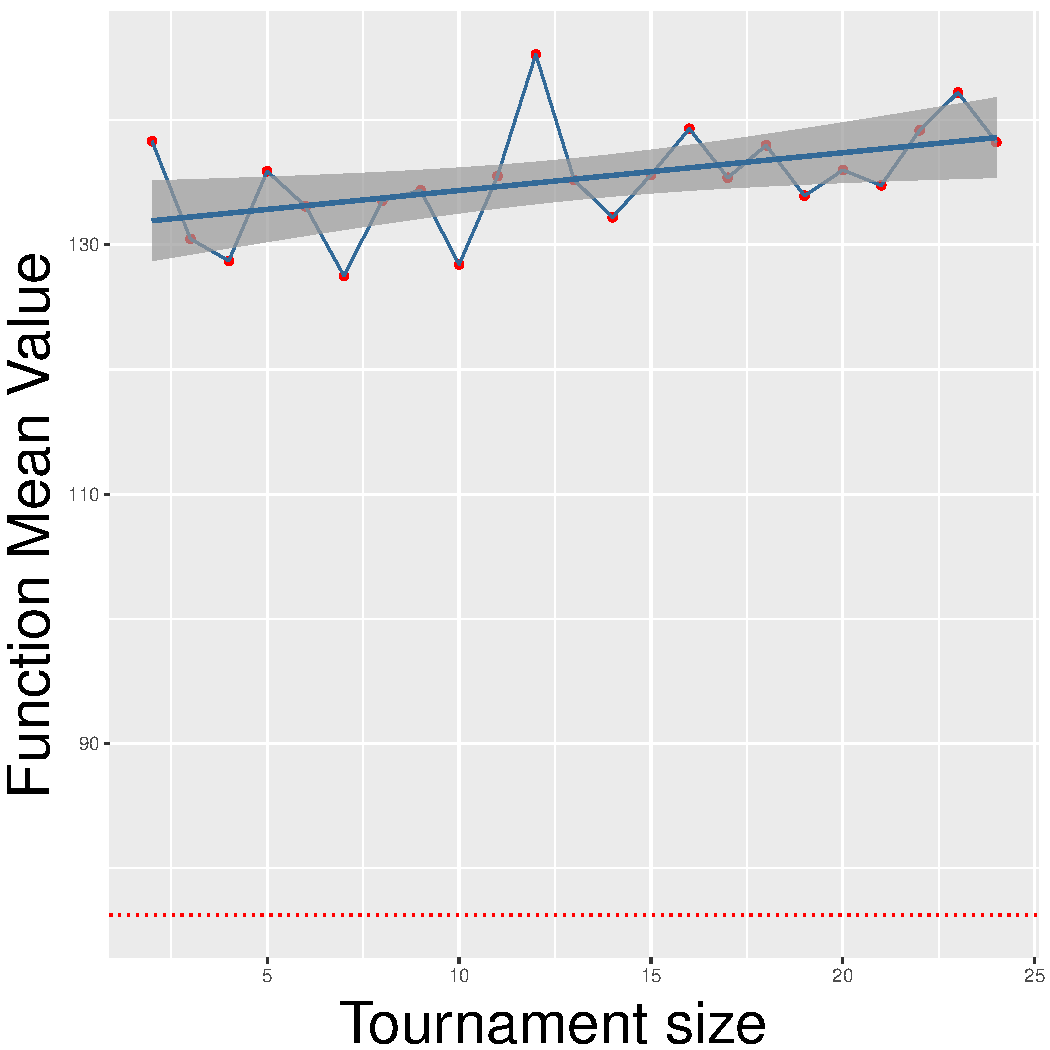
\includegraphics[width=\textwidth]{img/2n2n-40D/unimodal_2n2n_11_dim_40.pdf}
		\caption{40 dimensions.}
	\end{subfigure}
	\caption{Average performance on different tournament size for the Discus Function, when using the SBX crossover - ($\lambda + \lambda$) scheme.}
	\label{sbx-11-B}
\end{figure*}




\subsection{Overall Analysis}

The Friedman Test no significant difference for the unimodal functions with the uniform crossover, with any dimension. The test found significant difference for the multimodal functions, with higher values for the tournament size having better results, see Figure~\ref{uniform-22-a}.

On all other cases, the Friedman Test showed significant difference in values among tournament size. That is when the SBX operator is used, regarding the generational scheme, for every function (unimodal or multimodal).  


The results can be better analyzed in the following Tables~\ref{Friedman_test_uniform-a}, ~\ref{Friedman_test_sbx-a} and ~\ref{Friedman_test_sbx-b}.


\begin{table}[h]
	\centering
	\begin{tabular}{|l|l|l|l|}
		\hline
		\textbf{Function Group} & \textbf{Dimension size}      & \textbf{Chi-squared}        & \textbf{P-value}                     \\ \hline
		\multicolumn{1}{|l|}{Unimodal} & \multicolumn{1}{|l|}{10} & \multicolumn{1}{l|}{26.637} & \multicolumn{1}{l|}{0.2253} \\ \hline
		\multicolumn{1}{|l|}{Multimodal} & \multicolumn{1}{|l|}{10} & \multicolumn{1}{l|}{66.904} & \multicolumn{1}{l|}{2.012e-06}  \\ \hline
		\hline
		\multicolumn{1}{|l|}{Unimodal} & \multicolumn{1}{|l|}{20} & \multicolumn{1}{l|}{19.698} & \multicolumn{1}{l|}{0.6019} \\ \hline
		\multicolumn{1}{|l|}{Multimodal} & \multicolumn{1}{|l|}{20} & \multicolumn{1}{l|}{57.525} & \multicolumn{1}{l|}{5.152e-05}  \\ \hline
		\hline	
		\multicolumn{1}{|l|}{Unimodal} & \multicolumn{1}{|l|}{40} & \multicolumn{1}{l|}{22.3} & \multicolumn{1}{l|}{0.4421} \\ \hline
		\multicolumn{1}{|l|}{Multimodal} & \multicolumn{1}{|l|}{40} & \multicolumn{1}{l|}{37.091} & \multicolumn{1}{l|}{0.02312}  \\ \hline
	\end{tabular}
	\caption{Friedman Test results for Uniform Crossover - ($\lambda, \lambda$) scheme.}
	\label{Friedman_test_uniform-a}	
\end{table}


\begin{table}[h]
	\centering
	\begin{tabular}{|l|l|l|l|}
		\hline
		\textbf{Function Group} & \textbf{Dimension size}      & \textbf{Chi-squared}        & \textbf{P-value}                     \\ \hline
		\multicolumn{1}{|l|}{Unimodal} & \multicolumn{1}{|l|}{10} & \multicolumn{1}{l|}{49.997} & \multicolumn{1}{l|}{0.000587} \\ \hline
		\multicolumn{1}{|l|}{Multimodal} & \multicolumn{1}{|l|}{10} & \multicolumn{1}{l|}{81.653} & \multicolumn{1}{l|}{8.645e-09}  \\ \hline
		\hline
		\multicolumn{1}{|l|}{Unimodal} & \multicolumn{1}{|l|}{20} & \multicolumn{1}{l|}{105.91} & \multicolumn{1}{l|}{5.893e-13} \\ \hline
		\multicolumn{1}{|l|}{Multimodal} & \multicolumn{1}{|l|}{20} & \multicolumn{1}{l|}{88.885} & \multicolumn{1}{l|}{5.302e-10}  \\ \hline
		\hline
		\multicolumn{1}{|l|}{Unimodal} & \multicolumn{1}{|l|}{40} & \multicolumn{1}{l|}{144.89} & \multicolumn{1}{l|}{< 2.2e-16} \\ \hline
		\multicolumn{1}{|l|}{Multimodal} & \multicolumn{1}{|l|}{40} & \multicolumn{1}{l|}{118.46} & \multicolumn{1}{l|}{3.316e-15}  \\ \hline
	\end{tabular}
	\caption{Friedman Test results for SBX Crossover - ($\lambda, \lambda$) scheme.}
	\label{Friedman_test_sbx-a}	
\end{table}

\begin{table}[h]
	\centering
	\begin{tabular}{|l|l|l|l|}
		\hline
		\textbf{Function Group} & \textbf{Dimension size}      & \textbf{Chi-squared}        & \textbf{P-value}                     \\ \hline
		\multicolumn{1}{|l|}{Unimodal} & \multicolumn{1}{|l|}{10} & \multicolumn{1}{l|}{54.011} & \multicolumn{1}{l|}{0.0001639} \\ \hline
		\multicolumn{1}{|l|}{Multimodal} & \multicolumn{1}{|l|}{10} & \multicolumn{1}{l|}{75.724} & \multicolumn{1}{l|}{8.073e-08}  \\ \hline
		\hline
		\multicolumn{1}{|l|}{Unimodal} & \multicolumn{1}{|l|}{20} & \multicolumn{1}{l|}{73.078} & \multicolumn{1}{l|}{2.15e-07} \\ \hline
		\multicolumn{1}{|l|}{Multimodal} & \multicolumn{1}{|l|}{20} & \multicolumn{1}{l|}{95.524} & \multicolumn{1}{l|}{3.867e-11}  \\ \hline
		\hline
		\multicolumn{1}{|l|}{Unimodal} & \multicolumn{1}{|l|}{40} & \multicolumn{1}{l|}{101.52} & \multicolumn{1}{l|}{3.502e-12} \\ \hline
		\multicolumn{1}{|l|}{Multimodal} & \multicolumn{1}{|l|}{40} & \multicolumn{1}{l|}{87.318} & \multicolumn{1}{l|}{9.762e-10}  \\ \hline
	\end{tabular}
	\caption{Friedman Test results for SBX Crossover - ($\lambda + \lambda$) scheme.}
	\label{Friedman_test_sbx-b}	
\end{table}



\subsection{Functions Analysis}

To get a finer intuition about the results, we show some visual examples, separated in two groups of Figures. The first group, shows the mean value achieved by the GA given a function. The second one, shows the convergence plot with the mean of the values found at each generation, the function target value with a given tournament size. All Figures represent the mean of 40 repetitions given a certain dimension.


The Figures~\ref{sbx-22-a} and ~\ref{uniform-22-a} exemplify that for the Gallagher's Gaussian 21-hi Peaks Function (with 10, 20 and 40 dimensions) changing the tournament size for higher values tend to increase the quality of the results, for the generational scheme ($\lambda, \lambda$). While for the generational scheme ($\lambda + \lambda$), the Figure~\ref{sbx-22-B} that exemplifies that for the Gallagher's Gaussian 21-hi Peaks Function changing the dimension has a dominating impact on the final values found by the GA. This means that for the same function but with different dimensions the values changing the tournament size may increase or decrease the quality of the results.

The dominance of the dimensionality observed in Figure~\ref{sbx-22-B} also occurs in the Discus Function. The Figures~\ref{sbx-11-a},~\ref{uniform-11-a}, (with 10, 20 and 40 dimensions) show  changing the dimensionality of the problem may have a high impact in the choice of the tournament value with the generational scheme ($\lambda, \lambda$). The Figure~\ref{sbx-11-B} show that with the generational scheme ($\lambda + \lambda$) changing the tournament size leads to significant better final values found by the GA. In this case it is understandable that smaller values may positive affect the results, specially with low dimensionality. 

For all Figures, the gray shaded area represents the 95\% confidence level interval for predictions from a linear model for each scenario showed and demonstrate that choosing small values for the tournament size, as 2 or 3 may be a very poor choice. For all Figures, the mean of 40 repetitions is shown as bullets and the red line is shows the objective target value for the function.


\subsection{Convergence Analysis}
To make sure that the GA is converging we show a few visual examples. The Figures~\ref{convergence-sbx-11-a}, ~\ref{convergence-uniform-11-a} exemplify that the for the Discus Function with 40 dimensions and with the SBX crossover and with the uniform crossover with the ($\lambda, \lambda$) scheme, respectively, while the Figure~\ref{convegence-11-b} exemplify for the same scenario the same with the ($\lambda + \lambda$) scheme. The GA is converging towards the optimum target value, represented by the bottom, red, horizontal line.


Similar Figures for other functions are available as supplementary materials.

